\documentclass[11pt]{article}

\usepackage[utf8]{inputenc}
\usepackage[T1]{fontenc}
\usepackage[a4paper,margin=1in]{geometry}
\usepackage{graphicx}
\usepackage{booktabs}
\usepackage{array}
\usepackage{float}
\usepackage{hyperref}
\usepackage{amsmath}
\usepackage{caption}
\usepackage{subcaption}
\usepackage{xcolor}

\hypersetup{
    colorlinks=true,
    linkcolor=blue,
    urlcolor=blue,
    citecolor=blue
}

\graphicspath{{report/figures/}{figures/}}

\title{\textbf{Solar Energy Production Forecasting with ARIMAX}\\
\large IE360 Time Series Analysis Term Project Report}
\author{Esad Talha Can\\
Boğaziçi University}
\date{May 2026}

\begin{document}
\maketitle

\begin{abstract}
This report presents a time-series forecasting pipeline for predicting next-day
hourly solar energy production. The project was developed as the IE360 Time
Series Analysis term project and ranked 2nd out of 30 groups in the project
performance evaluation. The final implementation combines historical solar
production, Open-Meteo weather forecasts, calendar variables, lagged production
features, and an ARIMAX-style SARIMAX model with exogenous regressors. The model
first forecasts total daily solar production and then distributes the daily total
into 24 hourly values using historical intra-day production profiles. A local
backtest around the last available production date produced a daily WMAPE of
7.44\% and an hourly WMAPE of 9.28\% over the recent evaluation window.
\end{abstract}

\section{Introduction}

Solar production forecasting is a practical time-series problem because the
observed production series depends on both temporal structure and exogenous
weather conditions. Solar output has a strong daily shape, seasonal variation,
and direct sensitivity to radiation and cloud cover. The objective of this
project is to forecast the next day's hourly solar production, denoted as
\texttt{sun\_rt}, and print the required result as a Python list of 24 values.

The final project code is implemented in \texttt{forecast.py}. The script fetches
production and weather data at runtime, constructs a leakage-aware feature
table, trains a SARIMAX model with exogenous variables, and returns the next-day
hourly forecast. The current cleaned version also separates the forecasting
pipeline into readable functions, making the project easier to inspect,
validate, and extend.

\section{Problem Definition and Output Constraint}

The target variable is hourly solar production:
\[
    y_t = \texttt{sun\_rt}_t.
\]
For each execution date, the model must generate one prediction for each hour of
the next day:
\[
    \hat{y}_{d+1,0}, \hat{y}_{d+1,1}, \ldots, \hat{y}_{d+1,23}.
\]

The output constraint is operationally simple but strict: the final printed line
of the script must be a Python list containing exactly 24 numeric values. The
model therefore needs to handle missing recent production data, future weather
rows, and possible API delays without breaking the final output format.

\section{Data Sources}

\subsection{Production Data}

The dependent variable is loaded from a Google Drive CSV file through
\texttt{get\_production\_data()} in \texttt{forecast\_helper.py}. The table
contains timestamped observations of \texttt{sun\_rt}. Timestamps are converted
to the \texttt{Europe/Istanbul} timezone before merging with weather data.

Table~\ref{tab:data_summary} summarizes the local report run. The production
data currently ends on 2025-05-27, while the report was generated on a later
execution date. For that reason, current next-day forecasts cannot be evaluated
against actual values yet; validation is performed by anchoring the pipeline
around the last observed production date.

\begin{table}[H]
\centering
\caption{Data coverage from the local report run.}
\label{tab:data_summary}
\begin{tabular}{lr}
\toprule
Metric & Value \\
\midrule
Hourly rows in constructed table & 38,712 \\
Observed hourly production rows & 29,832 \\
Production date range & 2022-01-01 to 2025-05-27 \\
Forecast table end date & 2026-06-01 \\
Daily rows after aggregation & 1,613 \\
Final model feature count & 16 \\
\bottomrule
\end{tabular}
\end{table}

\subsection{Weather Data}

Weather data is downloaded from Open-Meteo for two plant coordinates. The model
uses the following hourly weather variables:

\begin{itemize}
    \item temperature at 2 meters,
    \item shortwave radiation,
    \item cloud cover,
    \item relative humidity,
    \item weather code.
\end{itemize}

The script combines historical forecast data and current forecast data. When
timestamps overlap, historical rows are prioritized because they are treated as
the best available past forecast history for training.

\section{Preprocessing and Feature Engineering}

The model constructs a continuous hourly time index from 2022-01-01 through the
forecast day. Production data and weather data are merged into this timeline by
timestamp. A 3-day lag is then created:
\[
    \texttt{sun\_rt\_lag\_3days}_t = \texttt{sun\_rt}_{t-72}.
\]

This lag is used because the latest production observations may not be available
at the time a next-day forecast is required. Using a 72-hour shift is a simple
way to keep the model closer to a realistic operational setting.

Weather features from the two plant locations are summarized into location-level
aggregates. The most important derived weather feature is effective radiation:
\[
    \texttt{effective\_radiation}
    =
    \texttt{shortwave\_radiation\_mean}
    \times
    \left(1 - \frac{\texttt{cloudcover\_mean}}{100}\right).
\]

Hourly rows are then aggregated into a daily modeling table. Table~\ref{tab:feature_blocks}
shows the feature blocks in the final model.

\begin{table}[H]
\centering
\caption{Feature blocks used in the final SARIMAX model.}
\label{tab:feature_blocks}
\begin{tabular}{lr}
\toprule
Feature block & Number of features \\
\midrule
Weather and transformed weather variables & 7 \\
Lagged production & 1 \\
Day-of-week dummy variables & 7 \\
Trend index & 1 \\
\midrule
Total & 16 \\
\bottomrule
\end{tabular}
\end{table}

All continuous production and weather features used by the model are transformed
with \(\log(1+x)\). Negative values are clipped to zero before transformation.
This keeps zero-production periods valid and reduces the effect of very large
daily production totals.

\section{Missing Values}

Missing values are expected because production data ends before the live weather
forecast horizon, and future target values are naturally unavailable. Table
\ref{tab:missingness} reports missingness from the local report run.

\begin{table}[H]
\centering
\caption{Missing-value summary from the local report run.}
\label{tab:missingness}
\begin{tabular}{lr}
\toprule
Area & Missing rate \\
\midrule
Hourly production target & 22.94\% \\
Hourly weather raw columns & 0.00\% \\
Daily feature matrix & 0.00\% \\
Next-day forecast rows & 9.52\% \\
\bottomrule
\end{tabular}
\end{table}

The important distinction is that missing future production values are not a
data-quality failure; they are the values the model is supposed to forecast.
Weather variables were complete in this run, while some forecast-day fields are
missing because they depend on future or lagged production values.

\section{Exploratory Analysis}

Figure~\ref{fig:daily_production} shows the last 365 observed days of daily
solar production. The series has strong seasonality and clear day-to-day
variation, which motivates combining lagged production with weather regressors.

\begin{figure}[H]
\centering
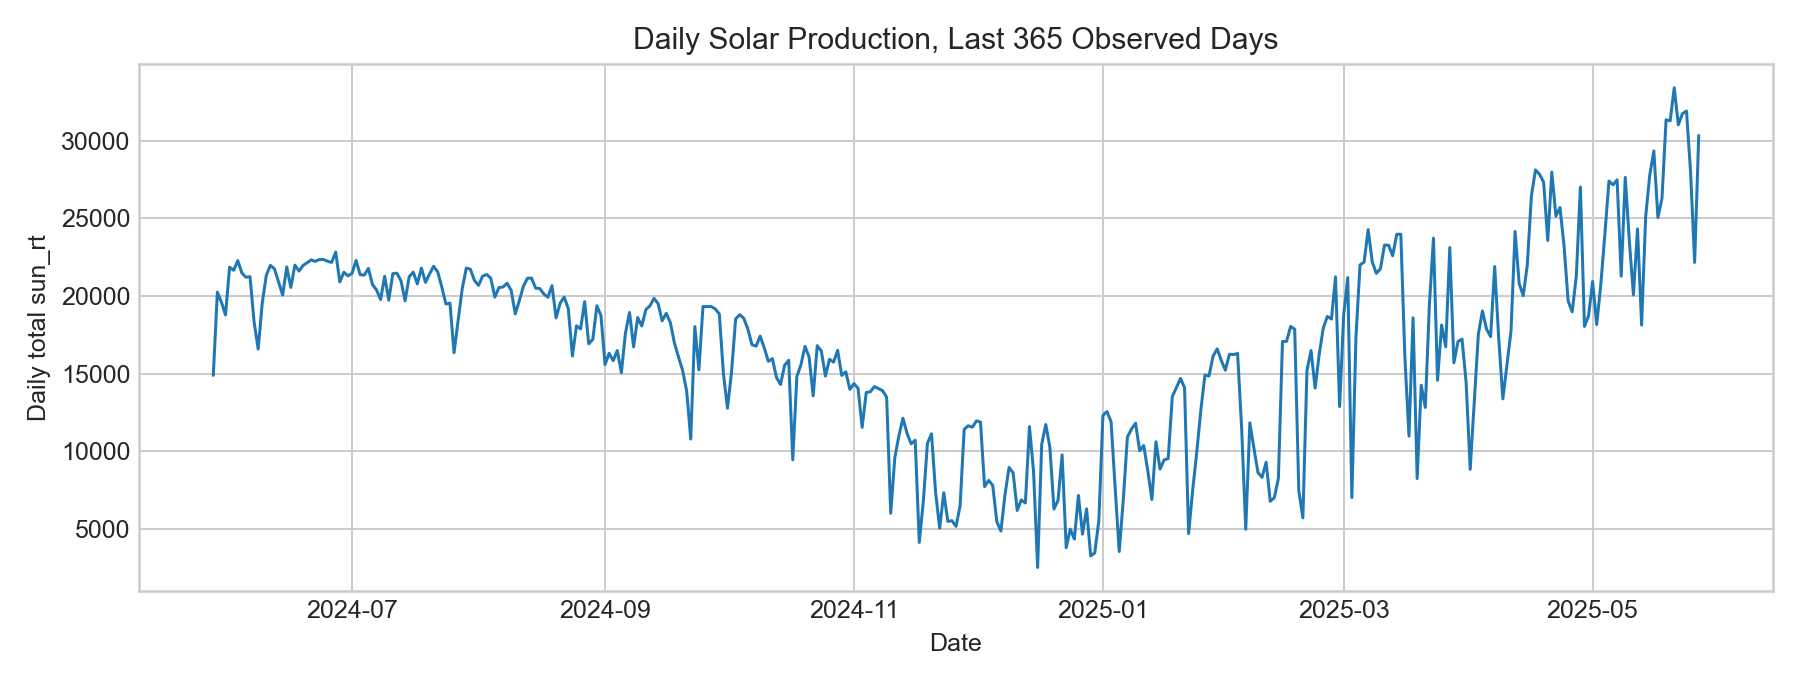
\includegraphics[width=0.95\textwidth]{daily_production.png}
\caption{Daily solar production over the last 365 observed days.}
\label{fig:daily_production}
\end{figure}

Table~\ref{tab:correlations} lists the strongest correlations with daily
production among engineered daily variables. The 3-day lag is the strongest
single predictor, while radiation-related variables are also positively
associated with production. Cloud cover is negatively correlated, as expected.

\begin{table}[H]
\centering
\caption{Top correlations with daily solar production.}
\label{tab:correlations}
\begin{tabular}{lr}
\toprule
Variable & Correlation with daily production \\
\midrule
3-day lagged production sum & 0.903 \\
Maximum shortwave radiation & 0.430 \\
Mean shortwave radiation & 0.420 \\
Effective radiation & 0.353 \\
Mean cloud cover & -0.312 \\
Mean temperature & 0.311 \\
\bottomrule
\end{tabular}
\end{table}

\begin{figure}[H]
\centering
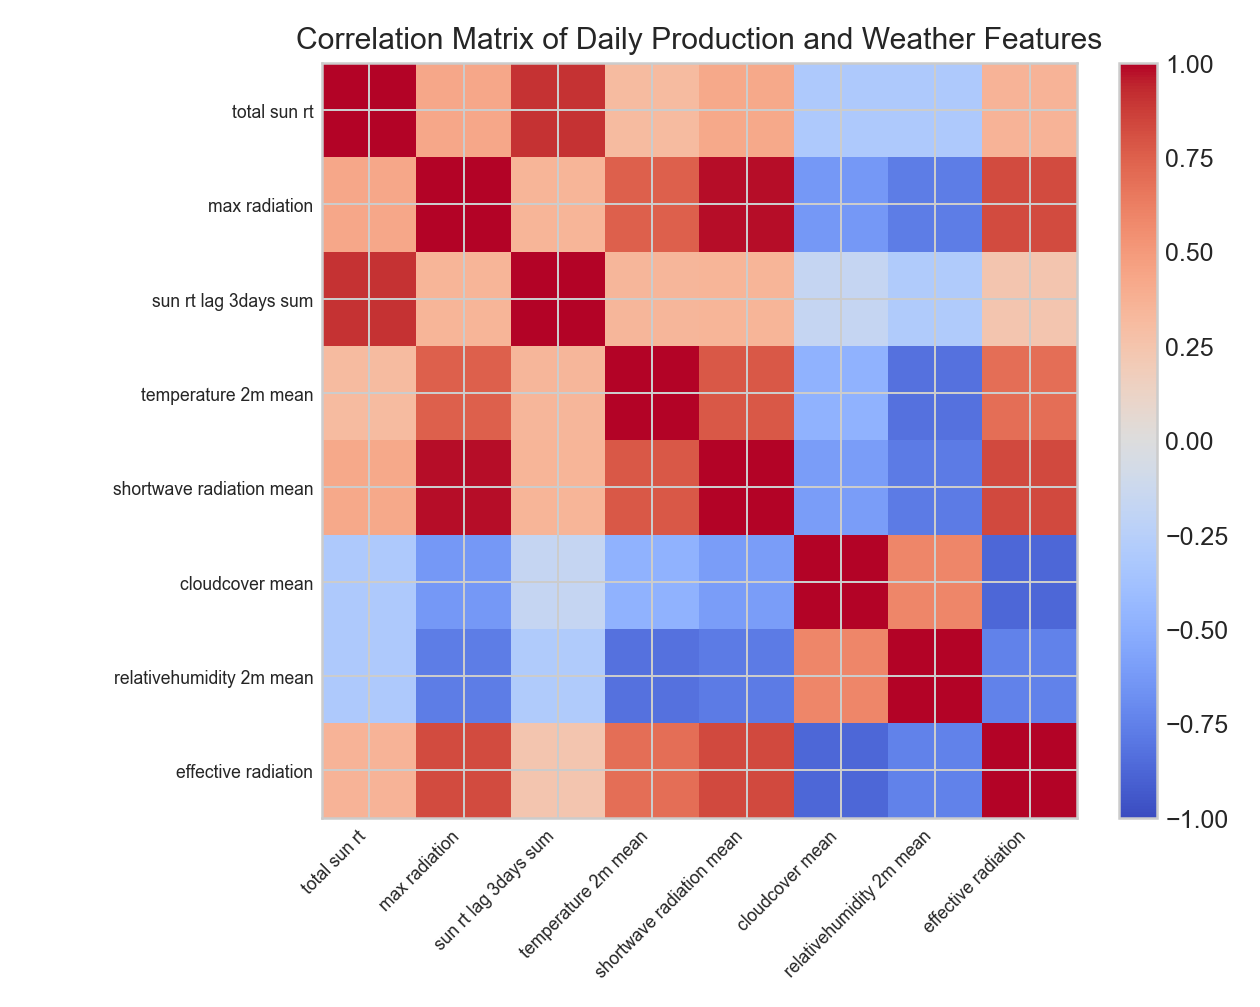
\includegraphics[width=0.78\textwidth]{correlation_matrix.png}
\caption{Correlation matrix for daily production and weather-derived variables.}
\label{fig:corr}
\end{figure}

\section{Modeling Approach}

\subsection{Daily ARIMAX-Style Model}

The final model uses SARIMAX as an ARIMAX-style model. The endogenous variable is
log-transformed total daily production. The exogenous regressors are the
engineered weather variables, the lagged production feature, day-of-week dummies,
and a trend index. The model order is:
\[
    (p,d,q) = (1,1,1).
\]

For a target day \(d+1\), training observations are restricted to dates up to
\(d-2\). This design avoids using production observations that would not be
known at forecast time.

\subsection{Hourly Distribution}

The SARIMAX model forecasts total daily production. The required output,
however, is hourly. To convert the daily forecast into 24 values, the pipeline
learns historical hourly production ratios:
\[
    r_{h} = \frac{\text{production at hour } h}{\text{daily production total}}.
\]

The ratios are grouped by year, ISO week, and hour. For a forecast date, the
matching weekly profile is used when available. If not available, the code falls
back to the previous week, then to the same ISO week averaged across years, and
finally to equal 24-hour allocation if no historical profile exists.

\begin{figure}[H]
\centering
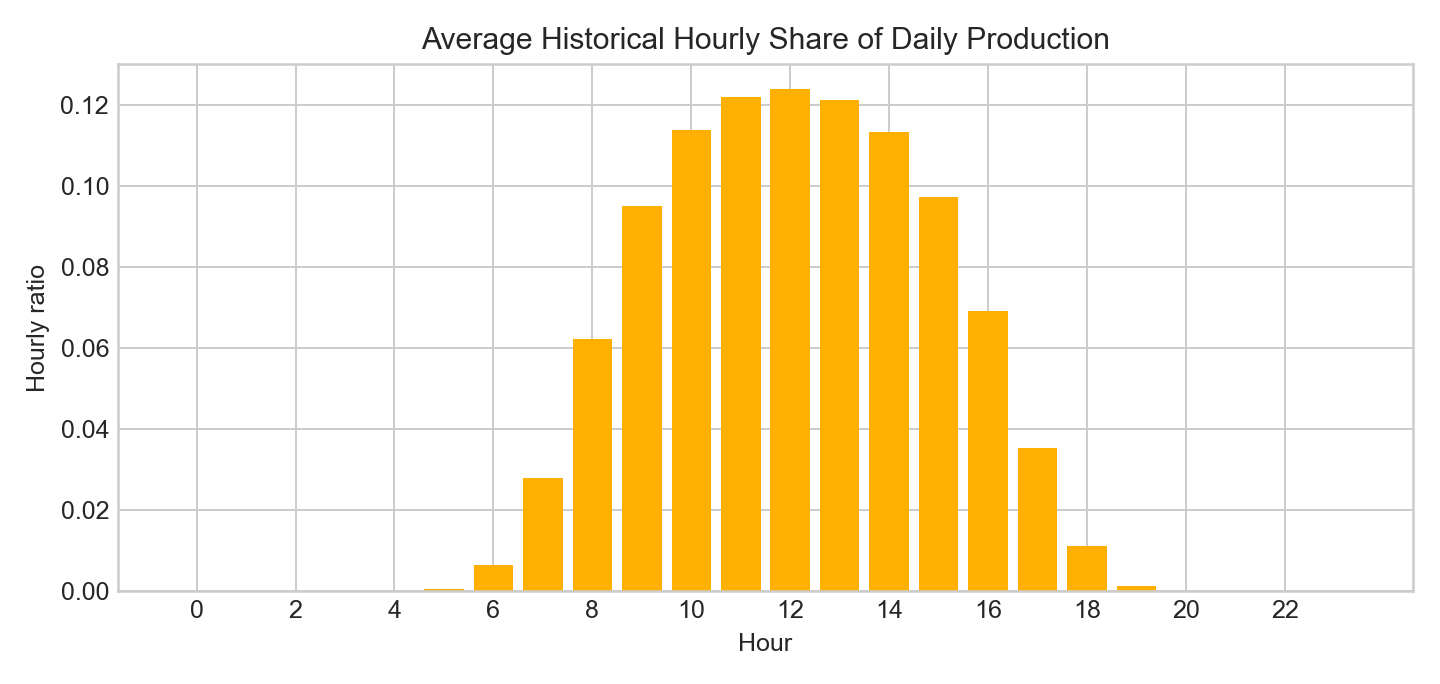
\includegraphics[width=0.85\textwidth]{hourly_profile.png}
\caption{Average historical hourly share of daily production.}
\label{fig:hourly_profile}
\end{figure}

\section{Validation Design}

Because the current hosted production data ends on 2025-05-27, live forecasts
for 2026-06-01 cannot be scored against actual production. To obtain a local
validation estimate, the pipeline was rerun with the forecast date fixed at
2025-05-27. The last 10 forecasted daily totals from that anchored run were then
compared with actual production values.

The main evaluation metric is WMAPE:
\[
    \text{WMAPE}
    =
    \frac{\sum_t |y_t - \hat{y}_t|}{\sum_t y_t} \times 100.
\]

MAE and RMSE are also reported for scale-aware interpretation.

\section{Results}

\begin{table}[H]
\centering
\caption{Backtest metrics around the last available production date.}
\label{tab:backtest_metrics}
\begin{tabular}{lrrrr}
\toprule
Level & Observations & MAE & RMSE & WMAPE \\
\midrule
Daily total forecast & 10 days & 2,214.96 & 2,566.09 & 7.44\% \\
Hourly forecast & 240 hours & 115.05 & 204.04 & 9.28\% \\
\bottomrule
\end{tabular}
\end{table}

Figure~\ref{fig:daily_backtest} compares the daily forecasts with actual daily
production in the recent validation window. The model follows the general level
of the production series, while individual daily errors remain due to weather
variation and the two-stage daily-to-hourly structure.

\begin{figure}[H]
\centering
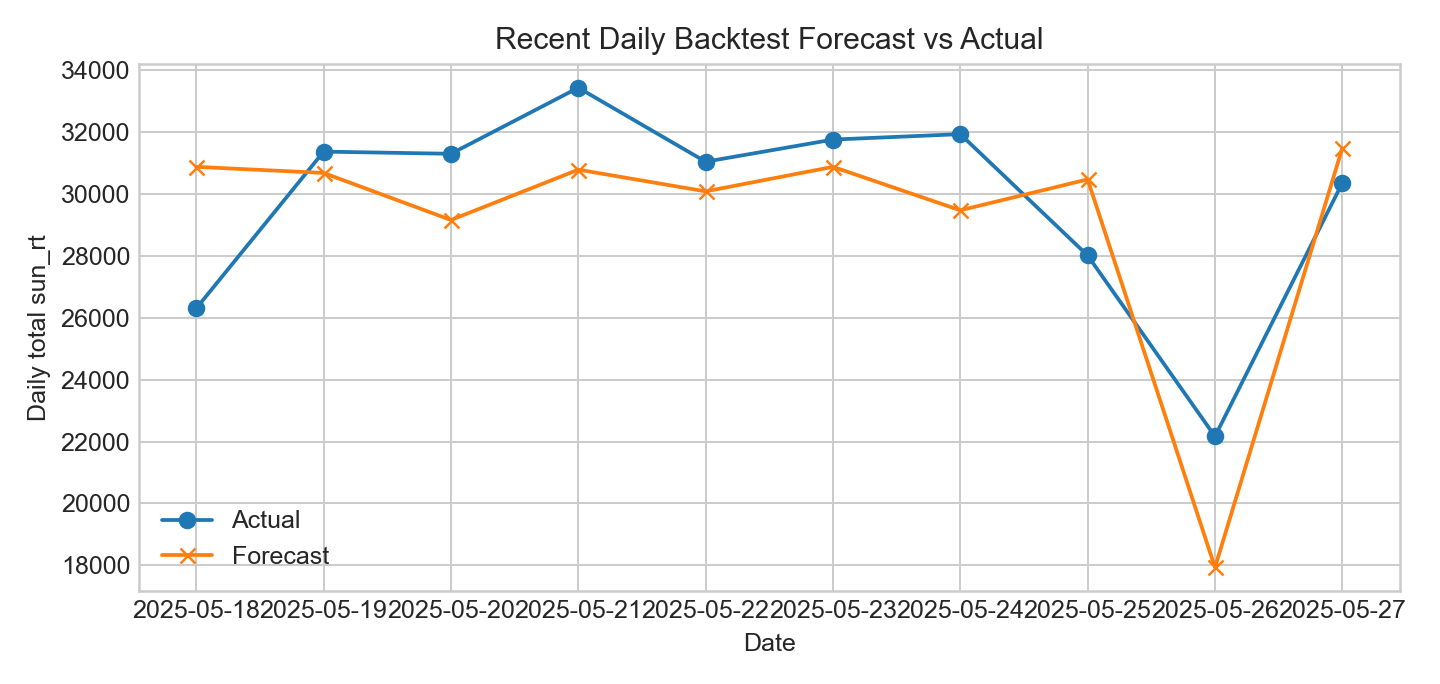
\includegraphics[width=0.9\textwidth]{daily_backtest.png}
\caption{Recent daily backtest forecast versus actual production.}
\label{fig:daily_backtest}
\end{figure}

\begin{figure}[H]
\centering
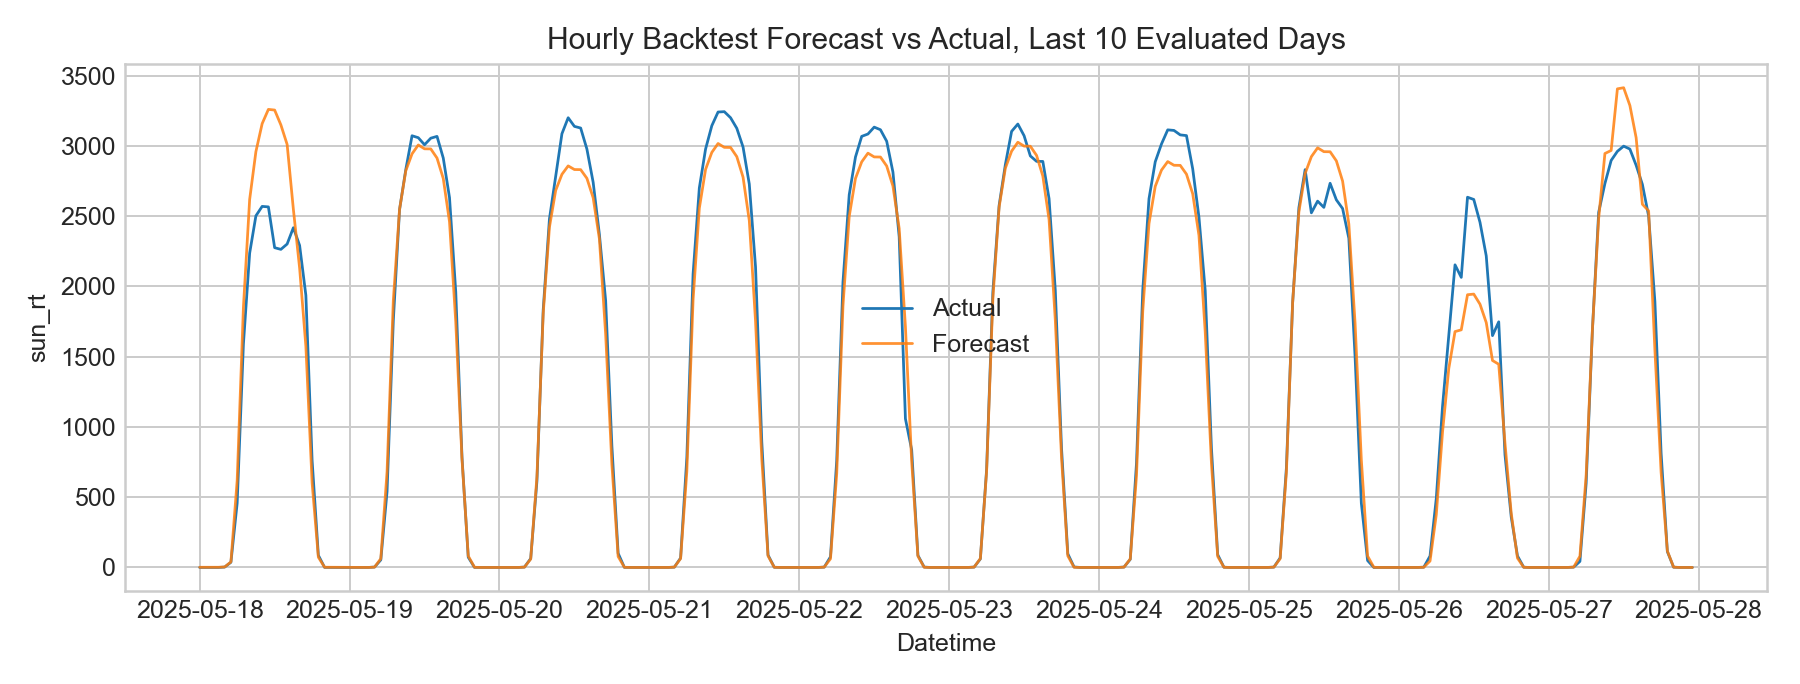
\includegraphics[width=0.95\textwidth]{hourly_backtest.png}
\caption{Hourly backtest forecast versus actual production for the evaluated period.}
\label{fig:hourly_backtest}
\end{figure}

\section{Operational Pipeline}

Table~\ref{tab:pipeline} summarizes the final implementation flow. The cleaned
code follows the same logical structure, with separate functions for data
loading, feature construction, daily forecasting, and hourly allocation.

\begin{table}[H]
\centering
\caption{Operational flow of \texttt{forecast.py}.}
\label{tab:pipeline}
\begin{tabular}{p{0.24\textwidth}p{0.44\textwidth}p{0.22\textwidth}}
\toprule
Step & Main action & Reliability note \\
\midrule
Load data & Fetch production and Open-Meteo weather data. & Weather and production are merged by timestamp. \\
Build features & Create lagged production, weather aggregates, effective radiation, trend, and weekday variables. & Uses lagged production to avoid same-day leakage. \\
Train daily model & Fit SARIMAX with exogenous regressors. & Model is retrained at runtime. \\
Forecast daily total & Predict future daily total on log scale and transform back. & Negative predictions are clipped to zero. \\
Distribute hourly & Apply historical hourly production ratios. & Falls back to previous week or same-week profile across years. \\
Print output & Return 24 numeric hourly forecasts. & Compatible with the project submission format. \\
\bottomrule
\end{tabular}
\end{table}

\section{Discussion}

\subsection{Strengths}

The final approach is interpretable and operationally practical. It uses domain
signals that are directly related to solar generation: shortwave radiation,
cloud cover, temperature, and historical production. The two-stage design also
reduces the burden on the SARIMAX model by forecasting daily totals instead of
modeling all hourly noise directly.

\subsection{Limitations}

The main limitation is data availability. The hosted production data currently
ends on 2025-05-27, so current 2026 forecasts cannot be scored unless updated
actual production is provided. The model also uses a fixed SARIMAX order rather
than automatically tuning \((p,d,q)\). Finally, the hourly allocation step is
heuristic: it uses historical ratios rather than a separate hourly regression
model.

\subsection{Possible Improvements}

The project could be improved by adding a reproducible local dataset, a
dedicated rolling backtest script, automatic SARIMAX parameter selection, and
alternative models such as regularized regression, random forests, or gradient
boosting. It would also be useful to refactor \texttt{forecast\_helper.py} to
remove duplicated weather API logic and to add command-line arguments for
forecast date and output path.

\section{Conclusion}

This project implements a complete next-day solar production forecasting
pipeline for the IE360 Time Series Analysis term project. The final model
combines historical production, weather forecasts, engineered calendar features,
and an ARIMAX-style SARIMAX model. The local backtest around the latest observed
production period produced 7.44\% daily WMAPE and 9.28\% hourly WMAPE. The
resulting implementation is compact, reproducible at runtime, and aligned with
the required 24-hour forecast output format.

\section*{References}

\begin{itemize}
    \item IE360 Time Series Analysis term project materials, Boğaziçi University.
    \item Open-Meteo Weather API: \url{https://open-meteo.com/}.
    \item Hyndman, R. J. and Athanasopoulos, G. \textit{Forecasting: Principles and Practice}.
    \item Durbin, J. and Koopman, S. J. \textit{Time Series Analysis by State Space Methods}.
    \item Statsmodels SARIMAX documentation: \url{https://www.statsmodels.org/}.
\end{itemize}

\end{document}
